\vspace{-2em}
\section{Αρχιτεκτονική}
\label{ArchitectureUsed_transfer}

Όπως έχει ήδη αναφερθεί η εκπαίδευση του μοντέλου για την πρόβλεψη των εικόνων τροφής του συνόλου δεδομένων FOOD101 έγινε με τη χρήση της τεχνικής της μεταφοράς μάθησης. Για τον λόγο αυτό χρησιμοποιήθηκε το εκπαιδευμένο μοντέλο ResNet50mod για εικόνες εισόδου μεγέθους (256, 256, 3) και πάνω σε αυτό έγιναν οι αλλαγές που απαιτούνταν ώστε να προχωρήσει η εκπαίδευσή του.

Η μορφή της αρχιτεκτονικής αυτού του μοντέλου φαίνεται στο σχήμα \ref{transfer_learning_fig}, το οποίο μοιάζει πολύ με αυτό του σχήματος \ref{Pretrained_Architectures_fig} με ουσιαστικές όμως διαφορές που οπτικοποιούνται από τα διαφορετικά χρώματα των πλαισίων του σχήματος.  

Πιο αναλυτικά, με μαύρο χρώμα παριστάνονται τα τμήματα της αρχιτεκτονικής του δικτύου που μένουν ακριβώς ίδια όπως αυτά εκπαιδεύτηκαν κατά την ανάπτυξη του μοντέλου ResNet50mod. Με κόκκινο χρώμα φαίνονται τα τμήματα τα οποία αλλάζουν προαιρετικά και για τα οποία όπως φαίνεται στο σχήμα \ref{Training_History_Transfer} εκτελέστηκαν δοκιμές. Πρόκειται για το επιπλέον τμήμα συνελικτικών επιπέδων που είχε προστεθεί επί του προ-εκπαιδευμένου ResNet50. Τέλος, με μπλε χρώμα φαίνονται τα επίπεδα τα οποία είναι καινούρια και τα οποία πρακτικά αντικαθιστούν τα εξωτερικά πλήρως διασυνδεδεμένα επίπεδα της ResNet50mod.  

Με βάση λοιπόν αυτήν την αρχιτεκτονική εκτελέστηκαν τρεις διαφορετικές αξιολογήσεις οι οποίες συνοψίζονται παρακάτω, ενώ σχηματοποιούνται στο σχήμα \ref{Training_History_Transfer}.

\begin{enumerate}
\item ResNet50mod\_transfer (1) : 0 ξεπαγωμένα layers σε σχέση με την αρχιτεκτονική ResNet50mod
\item ResNet50mod\_transfer (2) : Ξεπάγωμα των τριών εξωτερικών συνελικτικών layers σε σχέση με την αρχιτεκτονική ResNet50mod
\item ResNet50mod\_transfer (3) : Ξεπάγωμα και των έξι εξωτερικών συνελικτικών layers σε σχέση με την αρχιτεκτονική ResNet50mod
\end{enumerate}

Τέλος δίνεται και ο πίνακας \ref{parameters_transfer_table}, όπου φαίνεται ο αριθμός των προς εκπαίδευση παραμέτρων για κάθε μια από τις τρεις περιπτώσεις, η οποία εξηγεί και τον λόγο που το ξεπάγωμα των έξι συνελικτικών επιπέδων οδηγεί σε μεγαλύτερη ακρίβεια πρόβλεψης.

\begin{table}[H]
\centering
\begin{tabular}{|c|c|}
\hline
Περίπτωση                 & Αριθμός παραμέτρων προς εκπαίδευση \\ \hline
ResNet50mod\_transfer (1) & 570,469                            \\ \hline
ResNet50mod\_transfer (2) & 9,225,829                          \\ \hline
ResNet50mod\_transfer (3) & 23,386,213                         \\ \hline
\end{tabular}
\caption{Αριθμός προς εκπαίδευση παραμέτρων}
\label{parameters_transfer_table}
\end{table}


\begin{figure}[H]
\centering
\begin{subfigure}[t]{1.0\textwidth}%
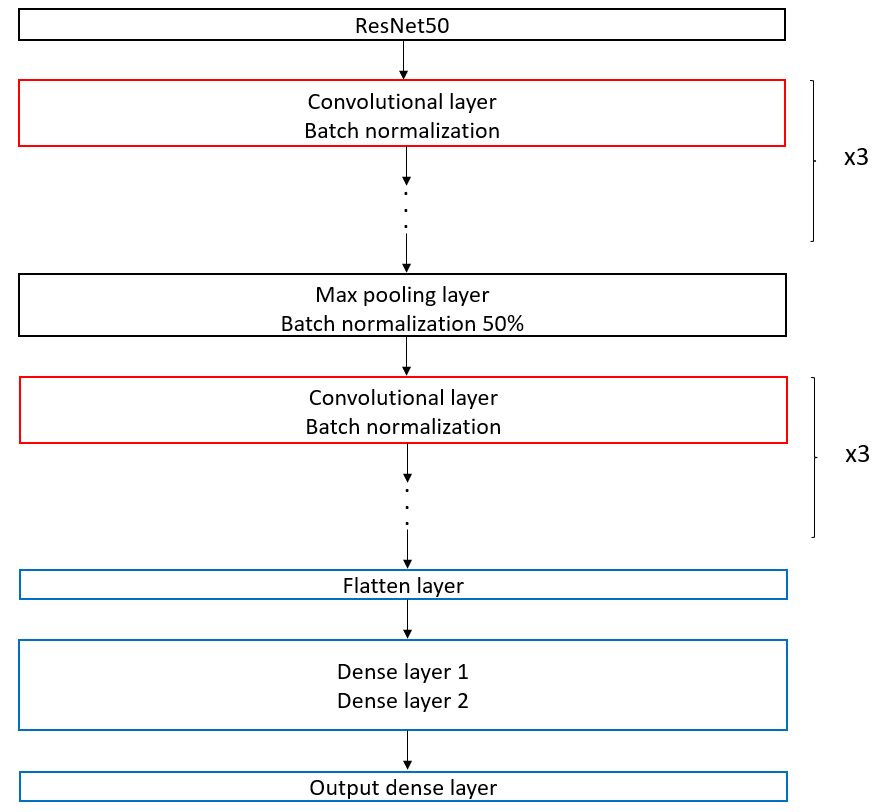
\includegraphics[width=\textwidth]{Transfer_Architecture.png}
\end{subfigure}
\caption{Αρχτιτεκτονική ResNet50mod (transfer learning)}
\label{transfer_learning_fig}
\end{figure}



\begin{figure}[H]
\centering
\begin{subfigure}[t]{1.0\textwidth}
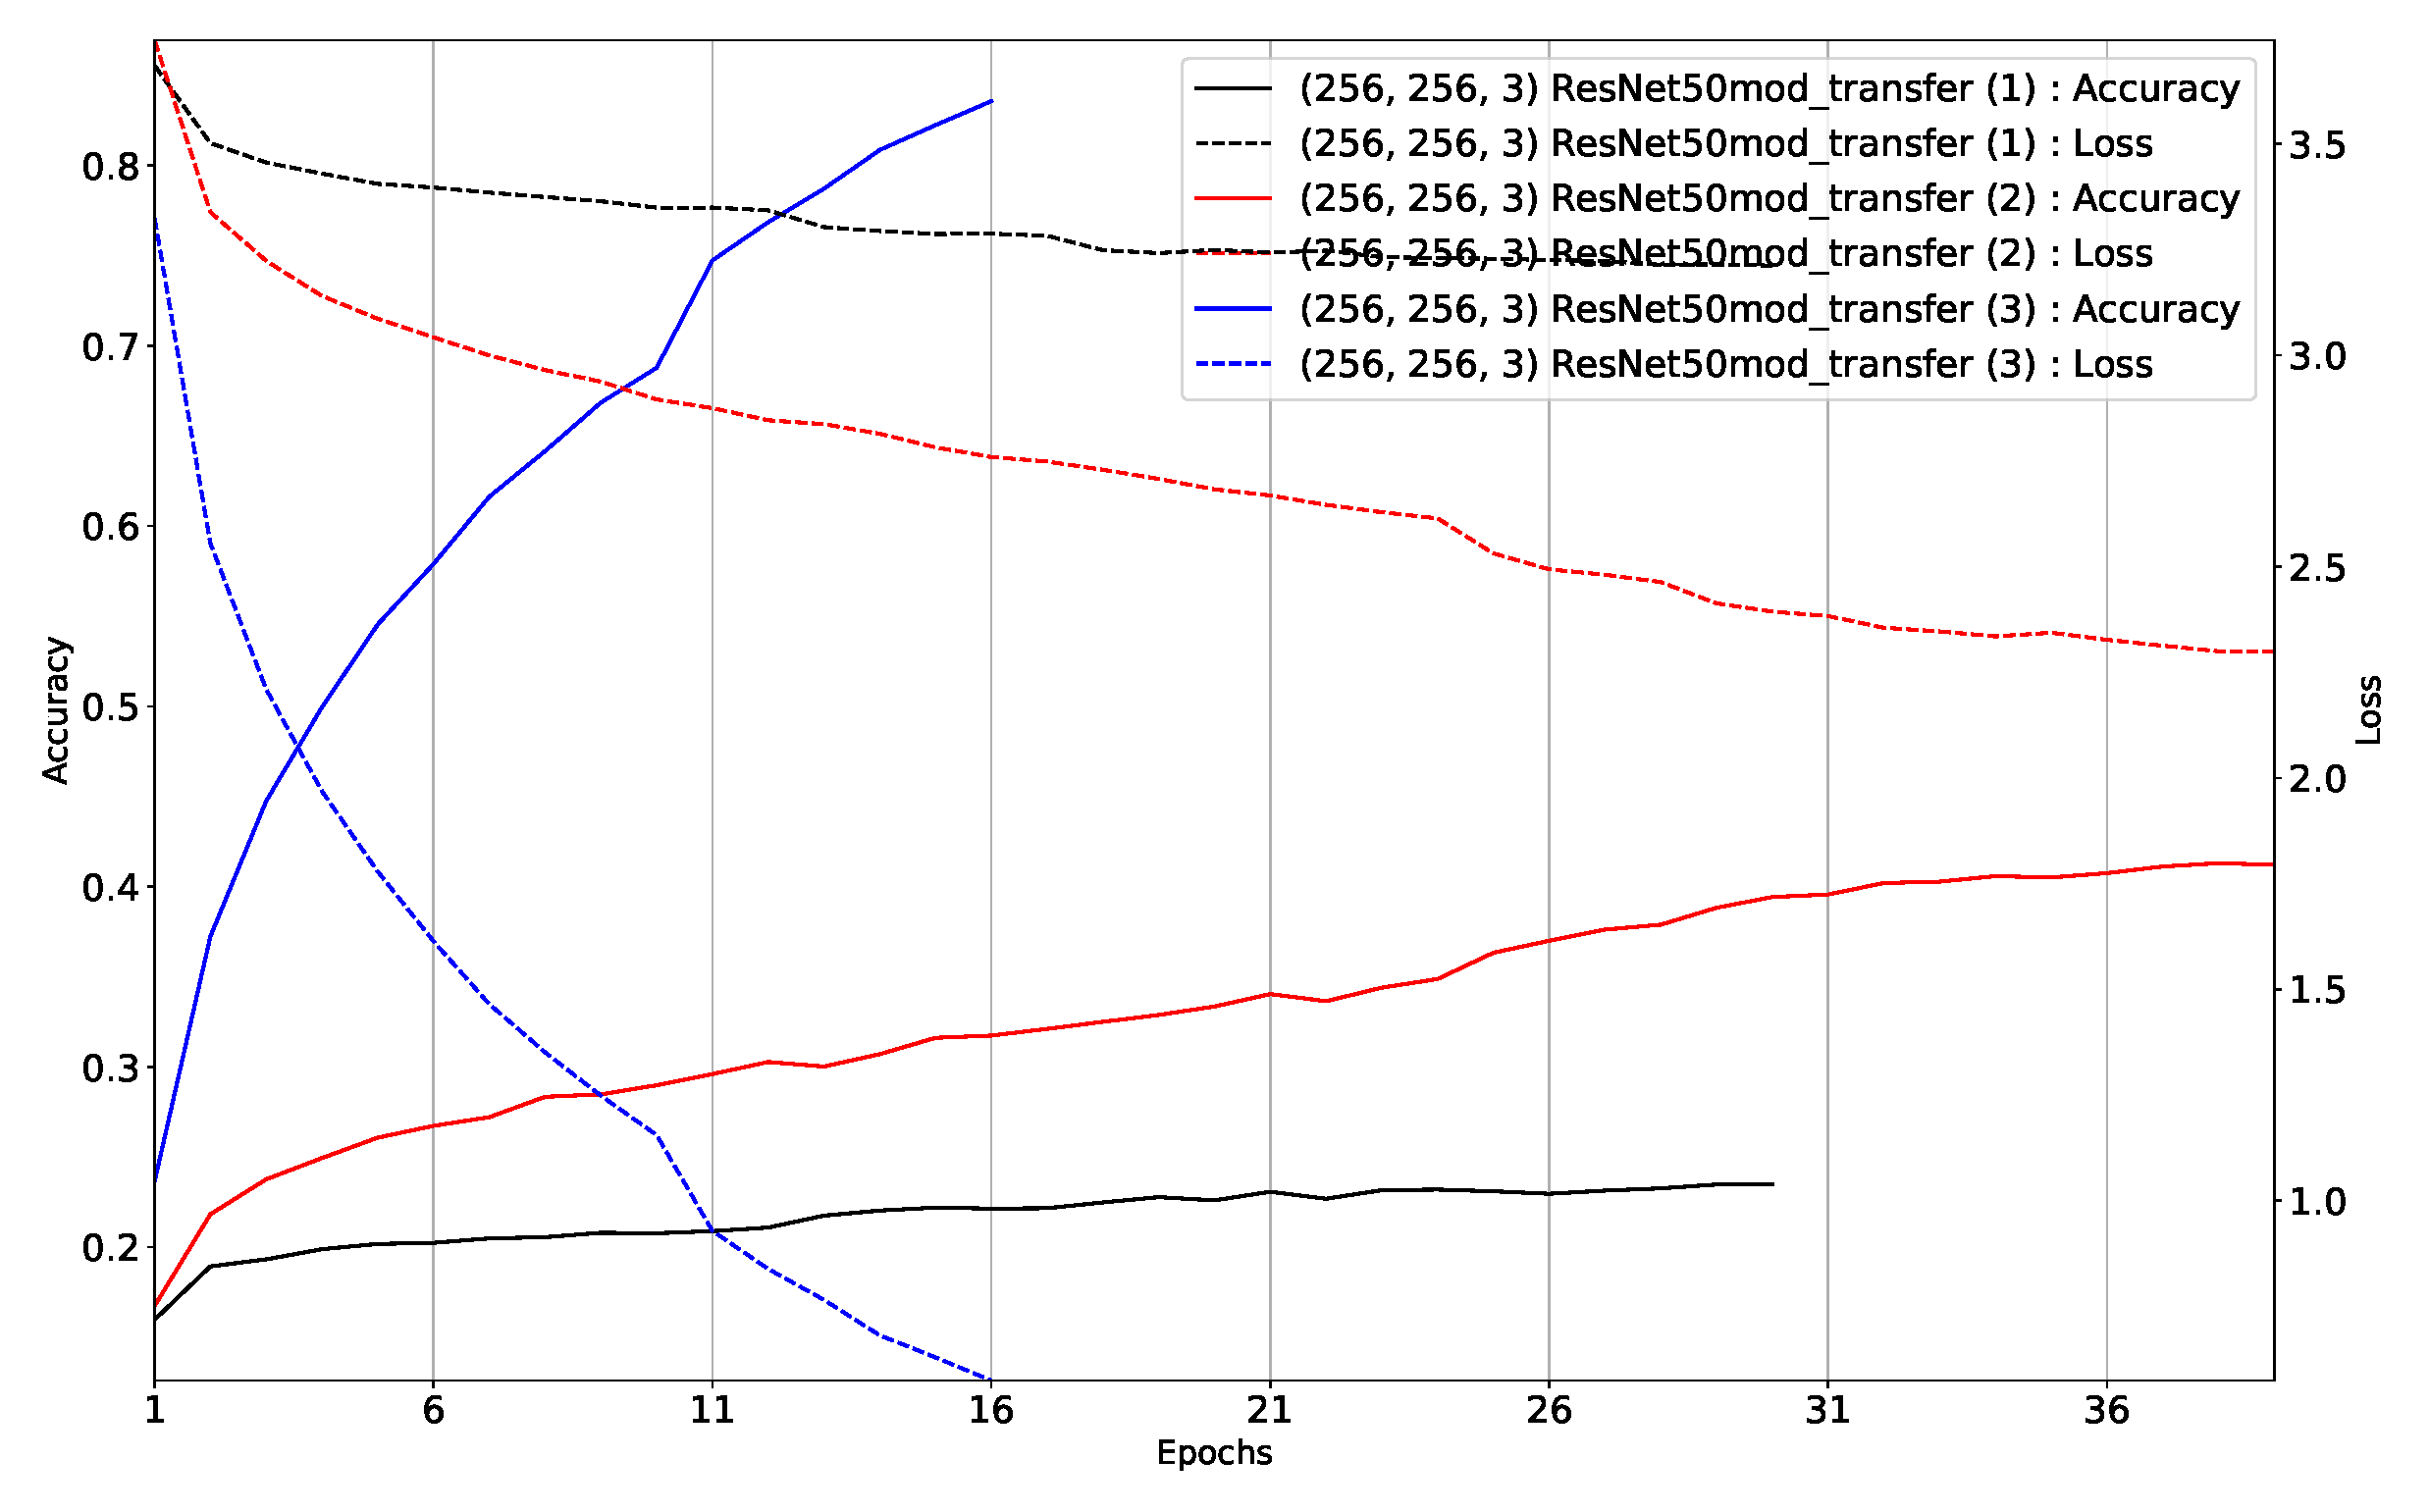
\includegraphics[width=\textwidth]{History_Transfer_Learning_Training.pdf}
\caption{Training}
\label{image_transfer_training}
\end{subfigure}
\begin{subfigure}[t]{1.0\textwidth}
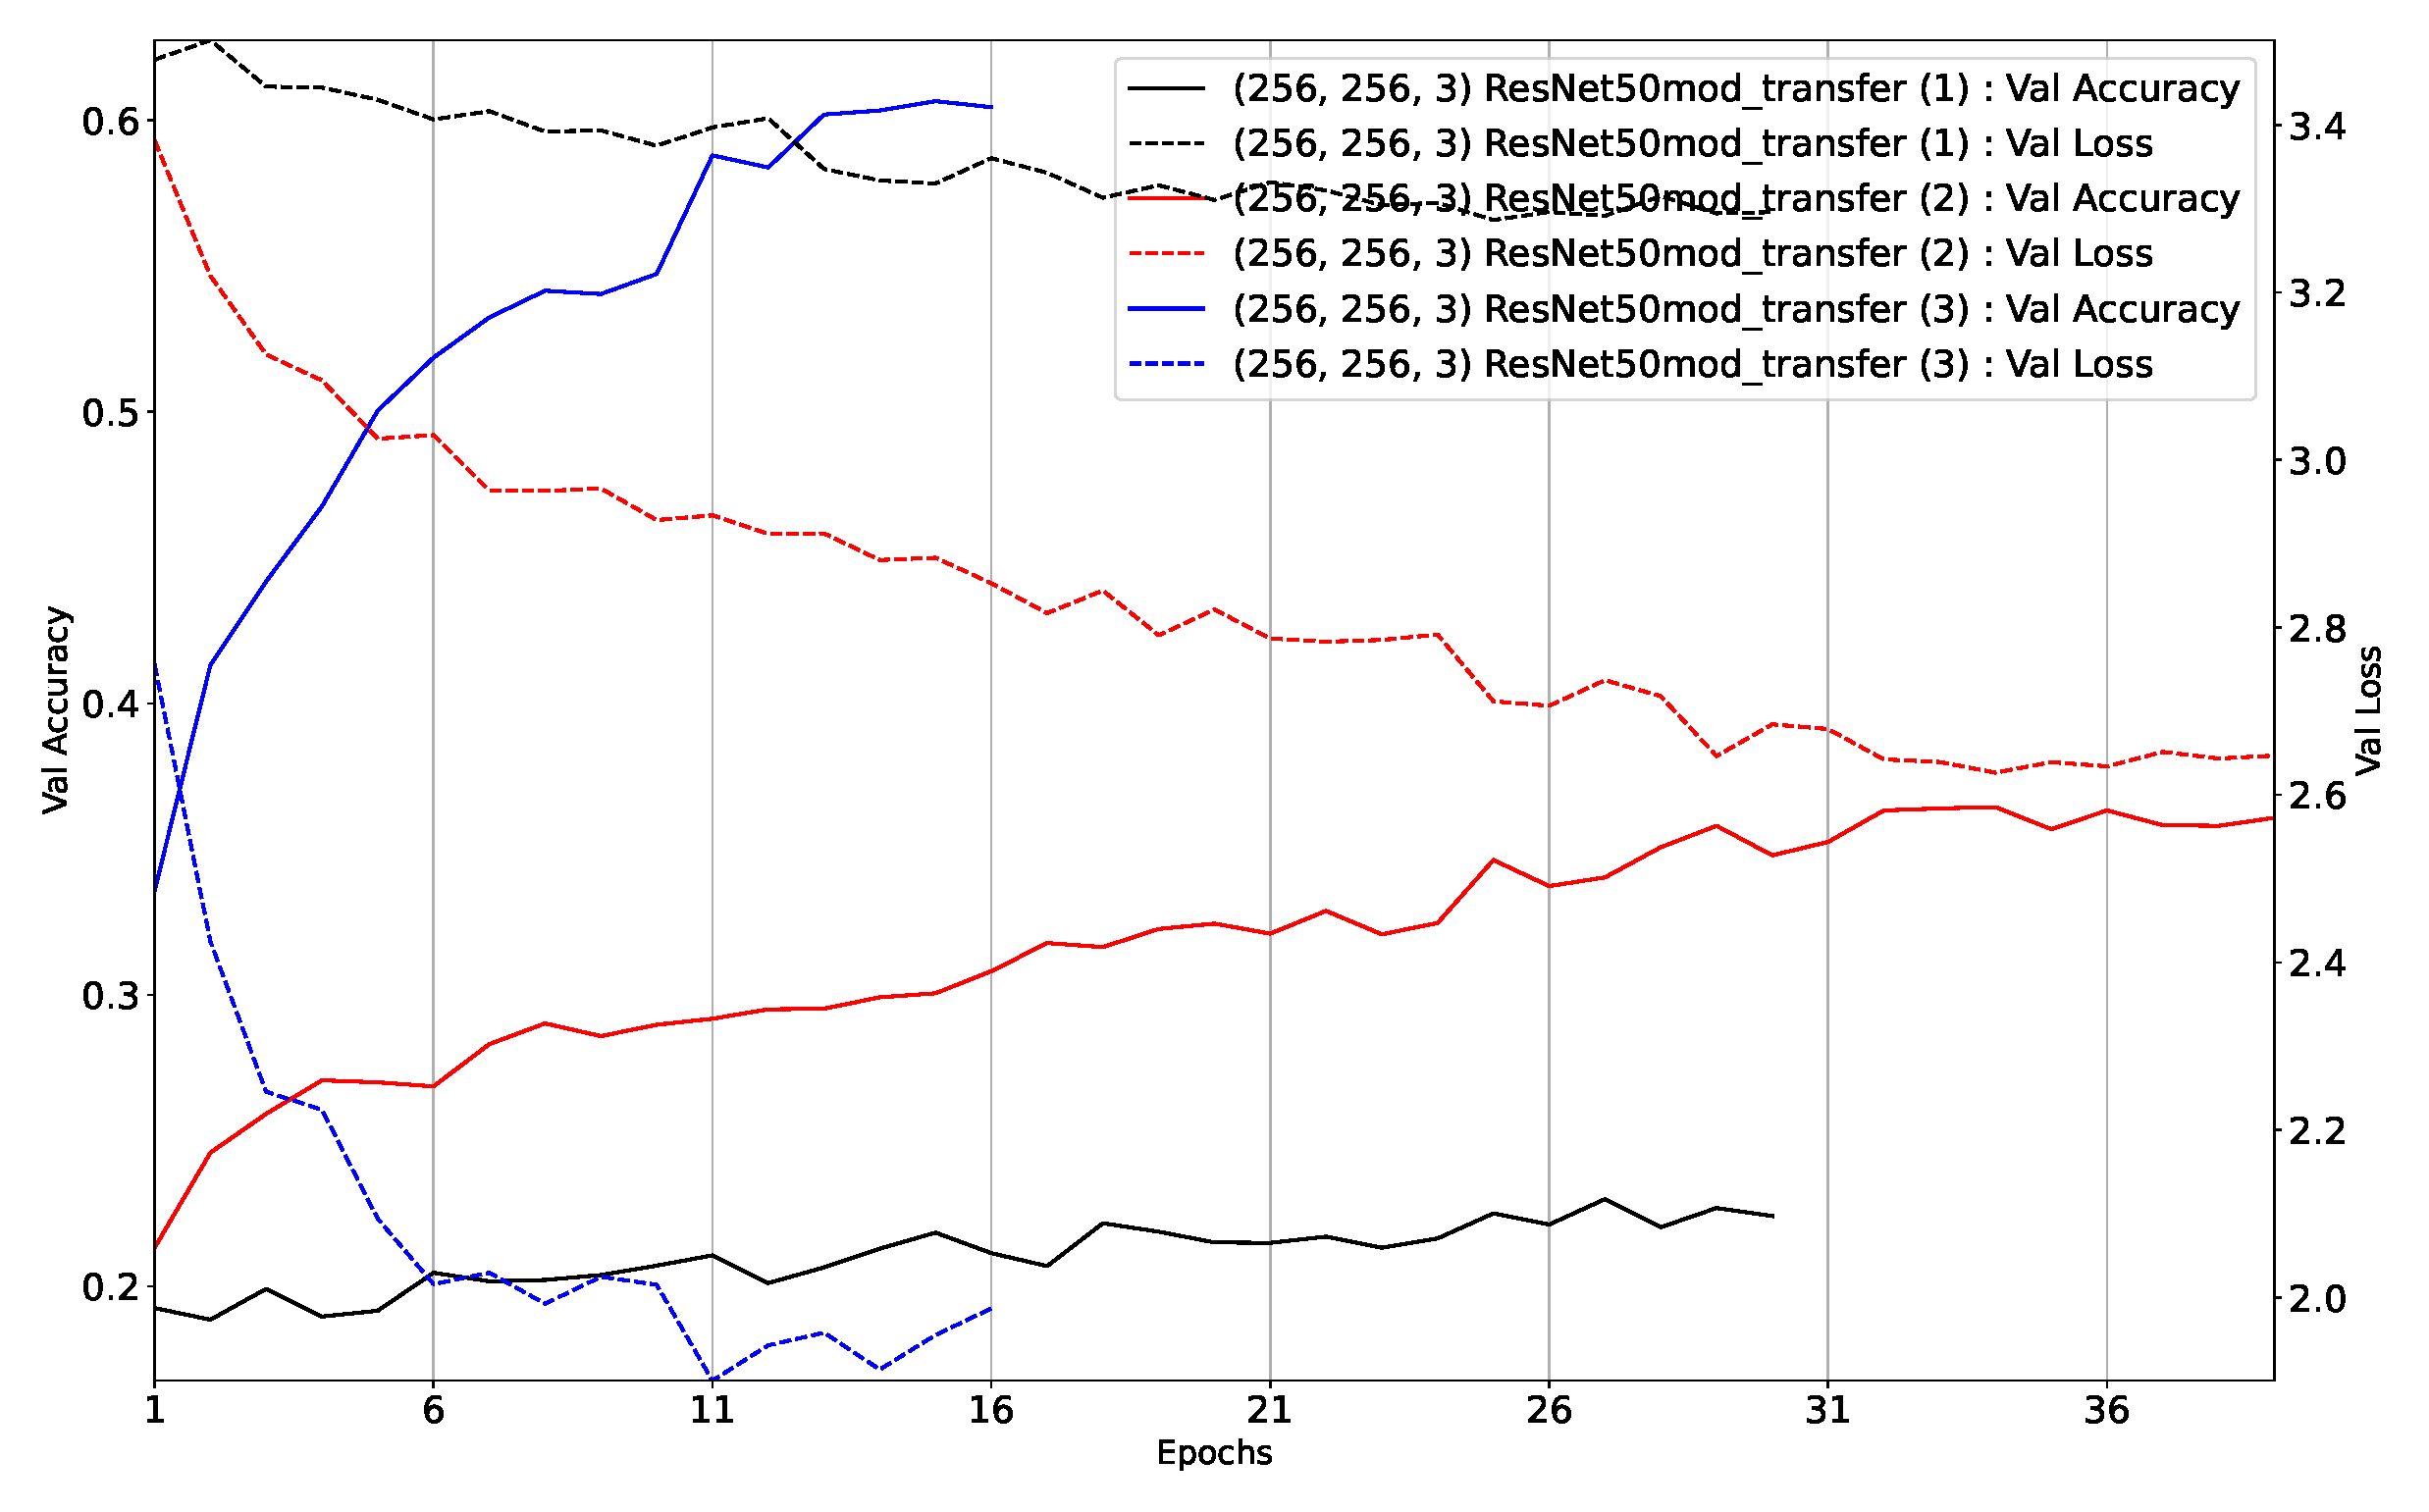
\includegraphics[width=\textwidth]{History_Transfer_Learning_Validation.pdf}
\caption{Validation}
\label{image_transfer_validation}
\end{subfigure}
\caption{Ιστορία εκπαίδευσης transfer learning}
\label{Training_History_Transfer}
\end{figure}



